\chapter{Vulnerability overview}
Table \ref{tbl:vuln overview} depicts all vulnerabilities found during the penetration test. They are categorized by their risk and potential and are differentiated in the categories low, medium, high and critical. 

Here describe what severities are and what do they mean in context of your report. It's better to keep the color code across all the report.

Figure  shows the overview of vulnerabilities grouped by target.

\begin{figure}[h]
\centering
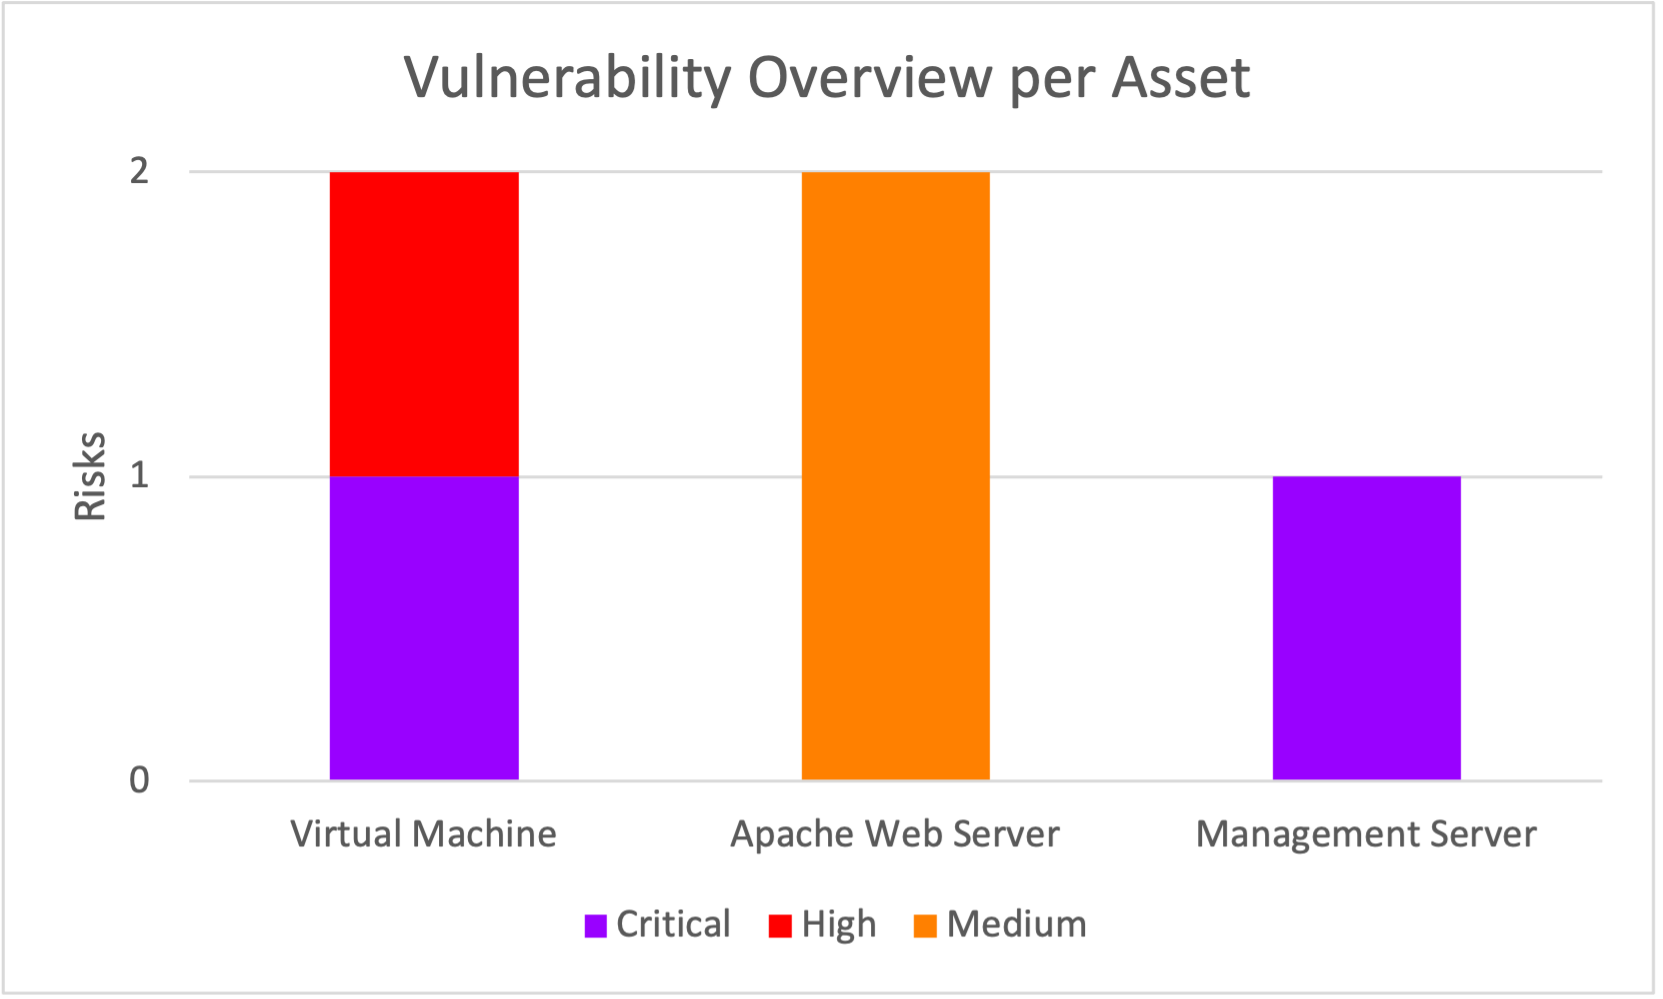
\includegraphics[width=\textwidth]{img/vulnerability_chart.png}
\caption{Vulnerability Overview}
\end{figure}

\begin{table}[h]
	\begin{tabular}{| l | l | p{7cm} | l | l |}
		\hline 
		Risk & Asset & Vulnerability & Section & Page\\
		\hline 
		\cellcolor{codepurple}Critical & Virtual Machine & Weak Password &  \ref{weak_password} & \pageref{weak_password} \\
		\hline 
		\cellcolor{red}High & Virtual Machine & Privilege Escalation &  \ref{privilege_escalation}& \pageref{privilege_escalation}\\
		\hline 
		\cellcolor{orange}Medium & Apache Web Server & Outdated Version &  \ref{outdated_version} & \pageref{outdated_version} \\
		\hline 
		\cellcolor{orange}Medium & Apache Web Server & Information Disclosure & \ref{information_disclosure} & \pageref{information_disclosure} \\
		\hline
		\cellcolor{codepurple}Critical & Management Server & Broken Authentication & \ref{management_server} & \pageref{management_server}\\
		\hline 
	\end{tabular}
	\caption{Vulnerability Overview}
	\label{tbl:vuln overview}
\end{table}